\section{Estimating DNA methylation variability in embryonic stem cells} \label{sec:bs}

\ifpdf
    \graphicspath{{Chapter3/bs/Figs/Raster/}{Chapter3/bs/Figs/PDF/}{Chapter3/bs/Figs/}}
\else
    \graphicspath{{Chapter3/bs/Figs/Vector/}{Chapter3/bs/Figs/}}
\fi

Several protocols have been developed for profiling average DNA methylation levels of in bulk populations of cells (\Cref{sec:intro_proto}). However, bulk profiling protocols are unable to directly estimate methylation heterogeneity between single cells, which is critical for studying embryonic development, cancer progression, and pluripotent stem cells. In the following, we will describe scBS-seq, an accurate and reproducible method for profiling DNA methylation in single cells, and a statistical model for estimating methylation heterogeneity in cell populations across the entire genome.


\subsection{Single-cell bisulfite sequencing protocol} \label{sec:bs_proto}

In commonly used BS-seq protocols, sequencing adaptors are ligated to fragmented DNA before bisulfite conversion, which results in a loss of information owing to DNA degradation by the bisulfite treatment. To minimize DNA loss from single cells, we developed a modification of post-bisulfite adaptor tagging~\citep{miura_amplification-free_2012-1}. In scBS-seq, bisulfite treatment is performed first, which results in simultaneous DNA fragmentation and conversion of unmethylated cytosines to thymine (\Cref{fig:bs_proto}). Then, synthesis of complementary strands is primed using oligonuleotides containing Illumina adaptor sequences and a 3' stretch of nine random nucleotides. This step is performed five times to maximize the number of tagged DNA strands and to generate multiple copies of each fragment. After capturing the tagged strands, a second adaptor is similarly integrated, and PCR amplification is performed with indexed primers.

\begin{figure}[htbp!]
\centering
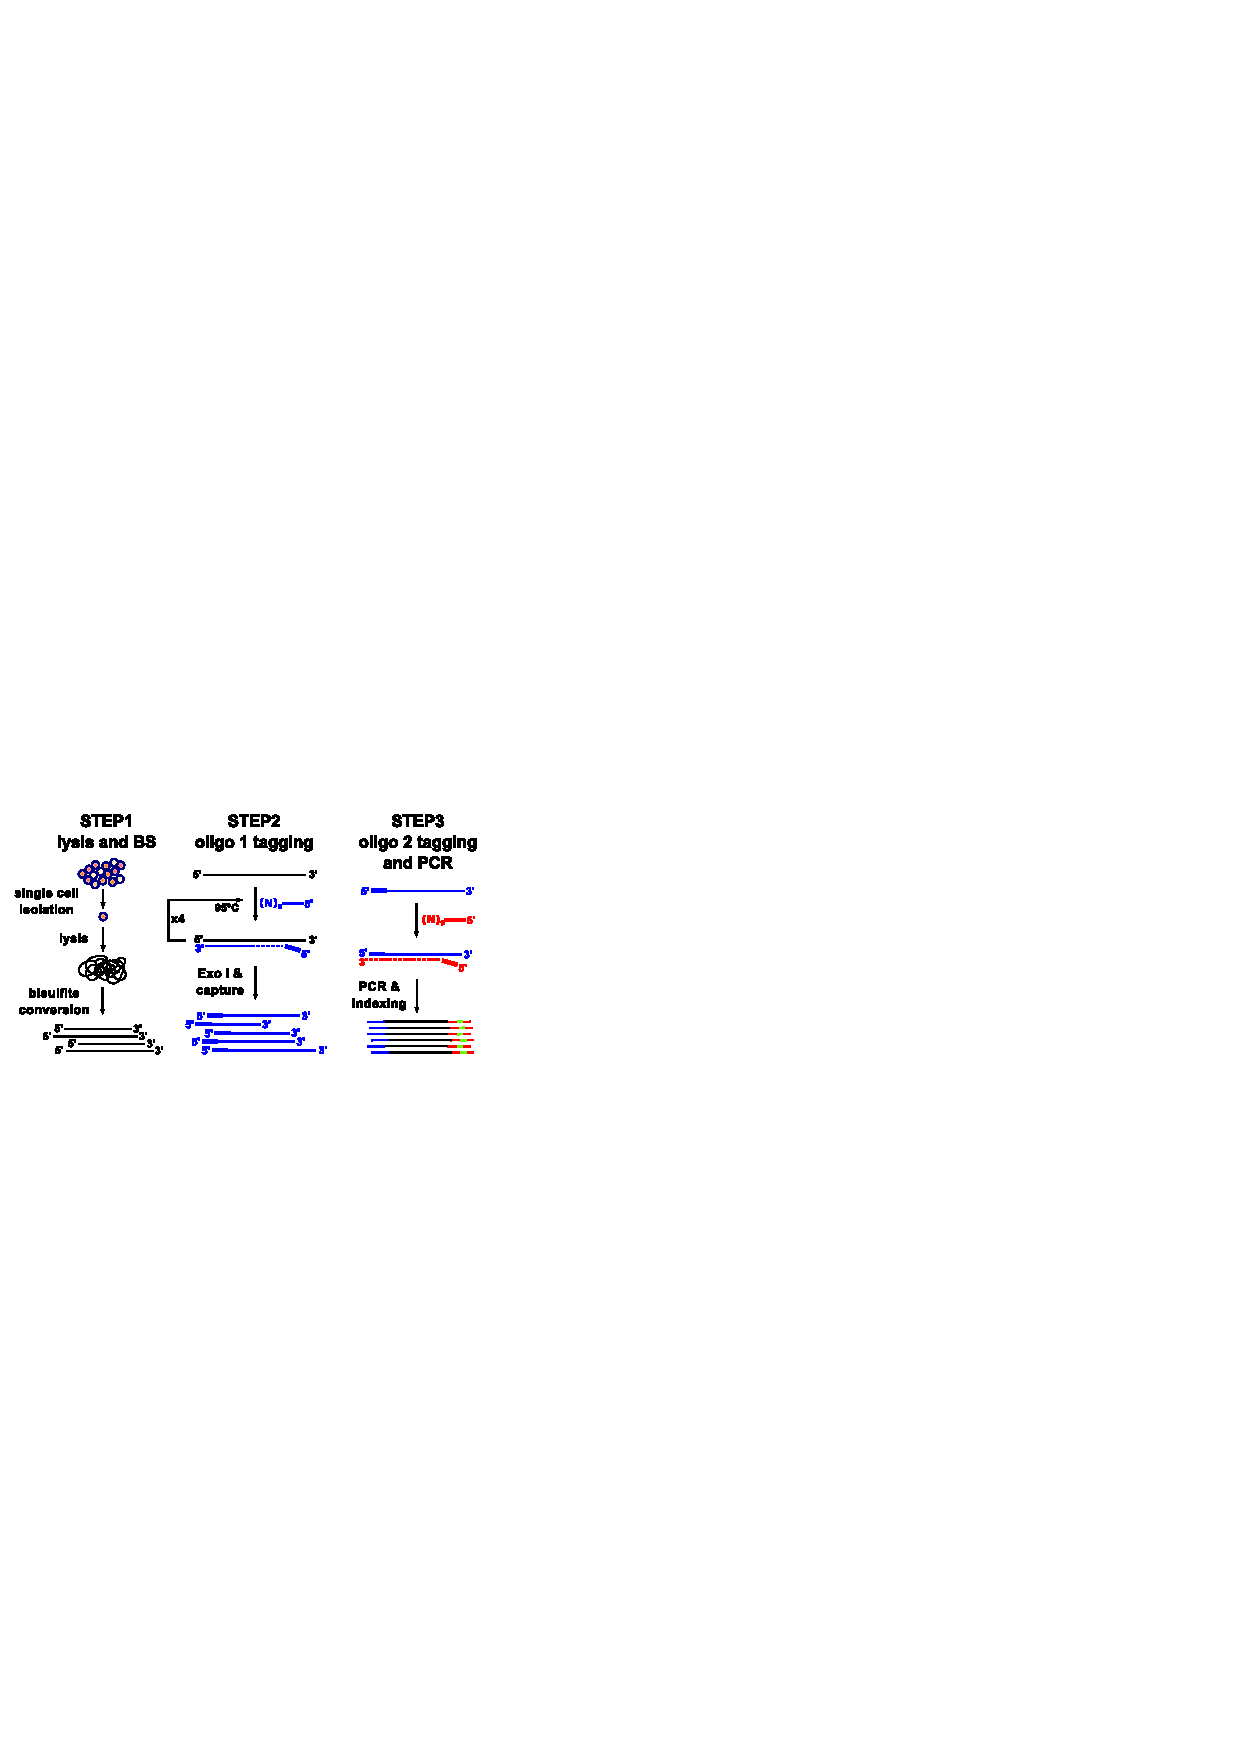
\includegraphics[width=0.75\textwidth]{proto}
\caption[scBS-seq profiling protocol.]{scBS-seq profiling protocol. scBS-seq library preparation consists of isolating and lysing single cells before bisulfite conversion (`BS'); performing five rounds of random priming and extension using oligo 1 (which carries the first sequencing adaptor) and purifying synthesized fragments; and performing a second random priming and extension step using oligo 2 (which carries the second sequencing adaptor) before amplifying the resulting fragments.}
\label{fig:bs_proto}
\end{figure}

We assessed scBS-seq on ovulated metaphase II oocytes (MIIs) and mouse ESCs cultured either in 2i medium or serum conditions. MIIs are a suited model for technical assessment as they: (i) can be individually hand- picked to ensure that only one cell is processed; (ii) represent a highly homogeneous population, which allows discrimination between technical and biological variability; and (iii) present a distinct DNA methylome comprising large-scale hypermethylated and hypomethylated domains~\citep{shirane_mouse_2013}. ESCs grown in serum conditions are characterized by a high heterogeneity in DNA methylation and gene expression and hence suited for the estimating of intercellular heterogenetiy~\citep{ficz_fgf_2013}. We used ESCs grown in serum (`serum ESCs') and ESCs grown in 2i medium (`2i ESCs') to determine whether scBS-seq can reveal DNA methylation heterogeneity in single cells.

We sequenced 12 MII, 12 2i ESC, 20 serum ESC, and 7 negative controls using scBS-seq, and their bulk cell counterparts using BS-seq. We obtained the methylation state of on average 3.7 million CpG dinucleotides (CpGs; range, 1.8 M–7.7 M) corresponding to 17.7\% of all CpGs (range, 8.5–36.2\%; \Cref{fig:bs_qc}~(a)). A higher CpG coverage can be obtained by deeper sequencing. To validate this, we sequenced two MII libraries close to saturation, which resulted in 1.5-fold and 1.9-fold more CpGs captured. Altogether, we obtained up to 10.1 M CpGs, corresponding to a CpG coverage of 48.4\%.

\begin{figure}[htbp!]
\centering
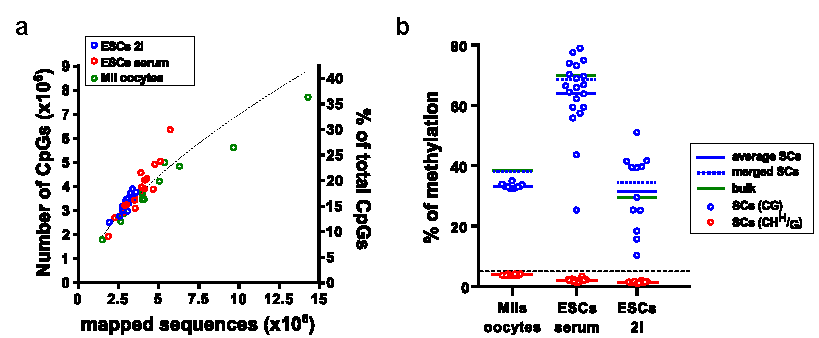
\includegraphics[width=0.8\textwidth]{qc}
\caption[scBS-seq mapping efficiency and mean methylation levels.]{scBS-seq mapping efficiency and mean methylation levels. (a) Number of CpGs obtained by scBS-seq as a function of mapped sequences. (b) Global mean DNA methylation levels in CpG (CG) and non-CpG (CHH/G) context for single cells (SCs), in silico–merged, and bulk samples. }
\label{fig:bs_qc}
\end{figure}

Next, we investigated the reproducibility and accuracy of scBS-seq. CpG sites in MIIs were overwhelmingly called methylated or unmethylated, which is consistent with a highly digitized output from single cells (\Cref{fig:bs_binary}). As expected, global methylation of MIIs was highly homogeneous ($33.1 \pm 0.8\%$) and 2i ESCs were hypomethylated compared to serum ESCs13. Yet both 2i ESCs and serum ESCs exhibited 5mC heterogeneity (serum, $63.9 \pm 12.4\%$; 2i medium, $31.3 \pm 12.6\%$; \Cref{fig:bs_qc}~(b)). We determined the average pairwise concordance between individual CpGs across single oocyte libraries, which was 87.6\% genome- wide (range, 85.3–88.9\%) and 95.7\% in unmethylated CGIs, a highly homogeneous genomic feature (\Cref{fig:bs_concord}~(a)). CpG concordance in ESCs was lower (serum, 72.7\%; 2i medium, 69.8\%), which reflected the heterogeneity of these cells (\Cref{fig:bs_concord}~(a)). At two kilo base pair (kbp) resolution, we observed high correlation between individual MIIs (Pearson's $r=0.92$), and between individual MIIs and bulk (Pearson's $r=0.95$) (\Cref{fig:bs_concord}~(b)). We could largely reproduce the entire bulk methylation profile of oocytes using only 12 single cells (\Cref{fig:bs_concord}~(b)). This capability is particularly beneficial for analyses of homogeneous cell populations and makes scBS-seq an important tool to investigate the 5mC landscape in very rare material.

\begin{figure}[htbp!]
\centering
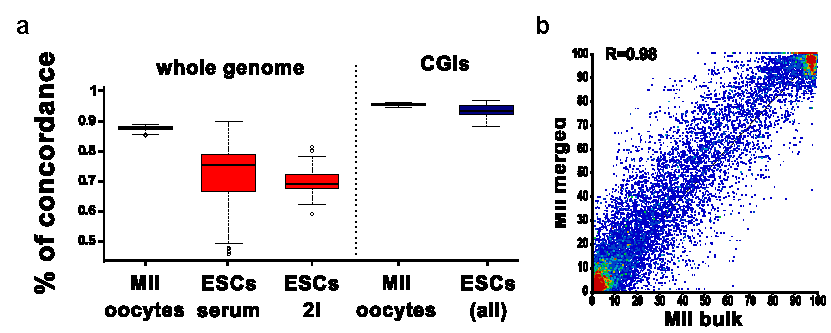
\includegraphics[width=1.0\textwidth]{concord}
\caption[scBS-seq concordance and reproduction of bulk data.]{scBS-seq concordance and reproduction of bulk data. (a) Pairwise analysis of CpG concordance genome-wide and in unmethylated CGIs. Boxplots represent the interquartile range, with the median; whiskers correspond to 1.5 times the interquartile range. (b) Pairwise correlation CpG methylation levels between MII-merged and MII-bulk data.}
\label{fig:bs_concord}
\end{figure}


\subsection{Method for estimating DNA methylation variability} \label{sec:bs_method}

The majority of CpG sites in single cells are either methylated or unmethylated. An exception is hemi-methylation, where the cytosine is methylated on only one DNA strand. Consistent with this, scBS-seq called CpG sites overwhelmingly methylated or unmethylated (\Cref{fig:bs_binary}). Since hemi-methylation is rare and currently hard to detect by scBS-seq owing to low CpG coverage, we did not consider hemi-methylation in our analysis. Instead, we modelled the methylation state of CpG sites in single-cells as a Bernoulli variable, and represented methylation profiles as a binary matrix (\Cref{fig:bs_binary}). As a consequence of the limited CpG coverage of only ${\approx}10-30\%$, the methylation state of most CpG sites is unobserved, which renders downstream analyses challenging. We therefore developed a method that aggregates information from adjacent CpG sites and estimates mean methylation levels as well as cell-to-cell heterogeneity for windows instead of single CpG sites. Our method yields uncertainty estimates, which is critical in regions of low CpG coverage. Our method is further computational efficient, thereby applicable genome-wide on over 20 million CpG sites.

\begin{figure}[htbp!]
\centering
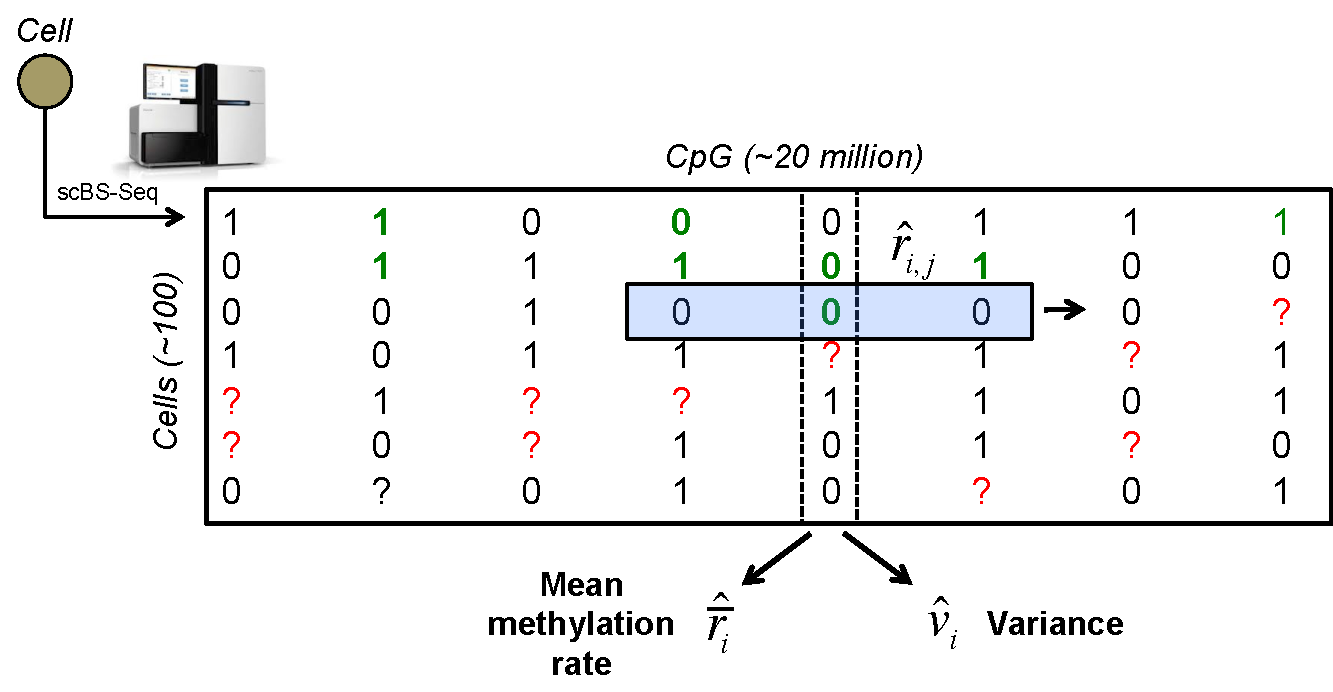
\includegraphics[width=0.9\textwidth]{method}
\caption[Representation of single-cell methylation data.]{Representation of single-cell methylation data. Binary matrix $M$ with rows corresponding to cells and columns to CpG sites. $M_{i,j}$ represent the methylation state of CpG site $i$ in cell $j$, which is one if the CpG site is methylated and zero otherwise. Question marks denote sites with unobserved methylation state. A sliding window (blue) is used to first estimate the methylation rate $\hat{r}_{i,j}$ (green) for each cell and window, and the mean methylation rate $\hat{\bar{r}}_i$ and variance $\hat{v}_i$ across cells afterwards.}
\label{fig:bs_method}
\end{figure}


\newcommand{\Xfw}{c^+}
\newcommand{\Xrv}{c^-}
\newcommand{\Xfws}{s^+_{i,j}}
\newcommand{\Xrvs}{s^-_{i,j}}
\newcommand{\XBin}{\operatorname{Bin}}
\newcommand{\Xse}{\operatorname{SE}}
\newcommand{\Xrij}{\hat{r}_{i,j}}
\newcommand{\Xri}{\hat{r}_i}
\newcommand{\Xwij}{w_{i,j}}
\newcommand{\Xrmi}{\hat{\overline{r}}_i}
\newcommand{\Xrvi}{\hat{v}_i}
\newcommand{\Xrvli}{\hat{v}^l_i}
\newcommand{\Xrvui}{\hat{v}^u_i}
\newcommand{\Xwjji}{w^{j,j^\prime}_i}


\subsubsection{Estimating cell-specific methylation rates}

To increase the coverage across cells, we employed a sliding window approach, which is conceptually similar to approaches that have been used for bulk BS-Seq~\citep{bock_dna_2012,li_dna_2010}. With window size $w=3000$~bp and step size 600~bp, we computed for each cell $j$ the sum of methylated $c^+_{i,j}$ and unmethylated $c^-_{i,j}$ read counts in window $i$:
\begin{align}
  \Xfws = \sum_{k=-w/2}^{+w/2} \Xfw_{i+k, j} \qquad
  \Xrvs = \sum_{k=-w/2}^{+w/2} \Xrv_{i+k, j}
\end{align}
To estimate methylation rates, we modelled the sum $S^+_{i,j}$ of methylated read counts as a Binomial random variable with methylation rate $r_{i,j}$:
\begin{align}
  S^+_{i,j}\sim \XBin(\Xfws+\Xrvs, r_{i,j})
\end{align}
Assuming $r_{i,j}\sim \operatorname{Beta}(1,1)$, leads to the maximum a posteriori estimator $\hat{r}_{i,j}$ of the methylation rate in cell $j$ and window $i$:
\begin{align}
  \Xrij = \frac{\Xfws+1}{\Xfws+\Xrvs+2}
\end{align}
To account for the limited CpG coverage of scBS-seq (\Cref{sec:bs_proto}), we quantified prediction uncertainty by approximating the standard error of the rate estimator using the Wald method~\citep{stein_sequential_1947}:
\begin{align}
  \Xse[\Xrij]^2 = \frac{\Xrij(1-\Xrij)}{\Xfws+\Xrvs}
\end{align}


\subsubsection{Estimating cell-to-cell variability}

We used the estimated cell-specific methylation rates $\Xrij$ to estimate the mean methylation rate and variance across all cells. We modelled the mean methylation rate $r_i$ in window~$i$ as a Gaussian random variable with mean $\overline{r}_i$ and variance $v_i$:
\begin{align}
  r_i \sim N(\overline{r}_i, v_i)
\end{align}
To account for differences in the standard errors $\Xse[\Xrij]$, we weighted cell $j$ and position $i$ by $\Xwij=\Xse[\Xrij]^{-2}$, and used the weighted maximum likelihood estimator
\begin{align}
  \Xrmi = \frac{1}{\sum_j \Xwij} \sum_j \Xwij\Xrij
\end{align}
to estimate $\overline{r}_i$. Its standard error is given by
\begin{align}
  \Xse[\Xrmi]^2 = \frac{1}{\sum_j \Xwij}.
\end{align}
The maximum likelihood estimator of the variance $v_i$ is
\begin{align} \label{eq:bs_var}
  \Xrvi = \frac{\sum_j \Xwij}{\left(\sum_j \Xwij\right)^2 - \sum_j \Xwij^2} \sum_j \Xwij \left(\Xrij - \Xrmi\right)^2,
\end{align}
which is the unbiased weighted cell-to-cell variance. The chi-squared confidence interval of the variance estimator with significance level $\alpha$ is
\begin{align}
  [\Xrvli, \Xrvui] = [\frac{n_i \Xrvi}{\chi^2_{1-\frac{\alpha}{2}, n_i}},
  \frac{n_i \Xrvi}{\chi^2_{\frac{\alpha}{2}, n_i}}].
\end{align}
Here, $\chi^2_{p, n_i}$ is the $p$-quantile of the chi-squared distribution with $n_i$ degrees for freedom, where $n_i$ is the sum of cell weights:
\begin{align}
  n_i^2 = \frac{\sum_j \Xwij}{\left(\sum_j \Xwij\right)^2 - \sum_j \Xwij^2}
\end{align}
To determine highly variable methylated sites, we ranked these by the lower bound $\Xrvli$ of the chi-squared confidence interval and defined the top k sites as the most variable sites. This approach is selecting sites with large estimates of cell-to-cell variance while penalizing for uncertainty of these estimates due to low CpG coverage.

\subsubsection{Cluster analysis}

To cluster cells and sites, we considered a complete linkage clustering, and employed the weighted Euclidean norm as distance measure for comparing cell $j$ with cell $j^\prime$:
\begin{align} \label{eq:bs_clust}
  d(j, j^\prime) = \sqrt{\sum_{i=1}^d \Xwjji \left(\hat{r}_{i,j} - \hat{r}_{i, j^\prime}\right)^2}
\end{align}
We defined the weight $\Xwjji$ at position $i$ as
\begin{align}
  \Xwjji \propto \sqrt{w_{i,j}w_{i,j^\prime}},
\end{align}
and normalized weights to sum up to the total number of positions $d$. This distance measure places most emphasis on positions that are covered by both cells.


\subsection{Methylation variability in different genomic contexts} \label{sec:bs_results}

\begin{figure}[htbp!]
\centering
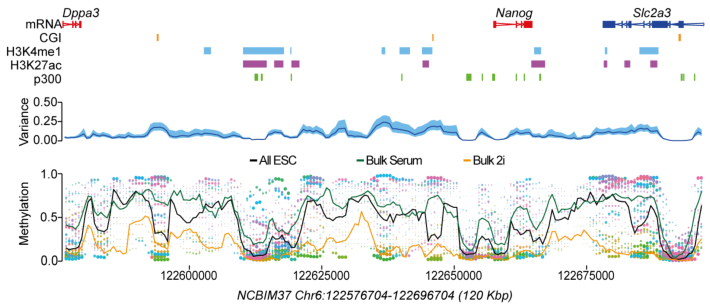
\includegraphics[width=1.0\textwidth]{zoom}
\caption[Estimated methylation rates for Nanog locus.]{Estimated DNA methylation rates using a sliding window in an example region containing the Nanog locus with some annotated features. Each single ESC is represented by a different color (bottom), and dot size is the inverse of estimation error. Mean methylation rate estimates across cells (black line, bottom) and cell-to-cell variance (blue line, middle; 95\% confidence interval in light blue) are shown. Methylation rates for `bulk serum' (green line) and `bulk 2i' (orange line) are superimposed (bottom).}
\label{fig:bs_zoom}
\end{figure}

We applied our method to estimate methylation rates in each ESC genome as well as the mean methylation rate and variance across all ESCs (\Cref{fig:bs_zoom}). By using our method for weighted clustering (\Cref{eq:bs_clust}), we identified two distinct clusters that represented the majority of 2i ESCs and serum ESCs (\Cref{fig:bs_clust}~(a)). Two outlier cells from the serum condition clustered with 2i ESCs, which implies that serum cultures contain `2i-like' ESCs and demonstrates the ability of scBS-seq to identify rare cell types in populations. To examine 5mC heterogeneity in ESCs in greater detail, we ranked sites by the estimated cell-to-cell variance (\Cref{eq:bs_var}) and repeated the cluster analysis for the 300 most variable sites (\Cref{fig:bs_top300}). The structure of the resulting clusters was broadly similar to what was observed based on genome-wide analysis, and all 300 variable sites followed the global trend of being more highly methylated in serum than 2i ESCs with high similarity between sites (\Cref{fig:bs_qc}~(b); \Cref{fig:bs_top300}). This observation is consistent with the genome-wide hypomethylation observed in ESCs grown in 2i medium~\citep{ficz_fgf_2013} and indicates that a major determinant of ESC heterogeneity is global methylation.

\begin{figure}[htbp!]
\centering
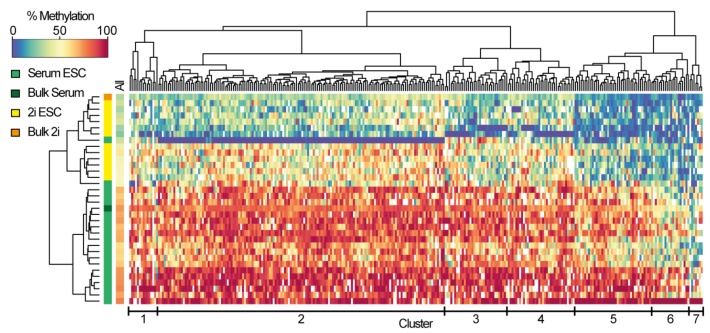
\includegraphics[width=1.0\textwidth]{top300}
\caption[Heatmap of top 300 most variable sites.]{Heatmap for methylation rates of the top 300 most variable sites among single-cell ESC samples. Cluster dendrograms for samples (left) and sites (top) are shown. The genome-wide average methylation rate is displayed in the left track (`all'). The main clusters of variable sites are indicated at the bottom.}
\label{fig:bs_top300}
\end{figure}

Our method also identified sites whose methylation varied more than the genome average, including sites with marked heterogeneity even among cells from the same growth condition (e.g. clusters 5 and 6 in serum ESCs; \Cref{fig:bs_top300}). Regions containing H3K4me1 and H3K27ac, marks associated with active enhancers, had the greatest variance in 5mC, whereas CGIs and intracisternal A-particle repeats had lower variance than the genome average (\Cref{fig:bs_clust}~(b)). These findings are consistent with observations that distal regulatory elements are differentially methylated between tissues and throughout development~\citep{stadler_dna-binding_2011,ziller_charting_2013,hon_epigenetic_2013}

\begin{figure}[htbp!]
\centering
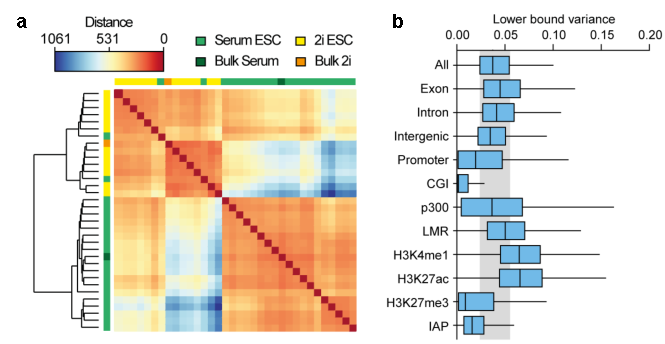
\includegraphics[width=1.0\textwidth]{clust}
\caption[Genome-wide clustering and estimated variance in genomic contexts.]{Genome-wide clustering and estimated variance in genomic contexts. (a) Genome-wide cluster dendrogram and distance matrix for all ESCs and bulk samples based on estimated methylation rates. Distance refers to the weighted Euclidean norm between estimated rates. (b) Variance of sites located in different genomic contexts. Boxes represent interquartile range with the median; whiskers correspond to 1.5 times the interquartile range. The shaded gray region indicates the interquartile range for all genome-wide sites.}
\label{fig:bs_clust}
\end{figure}
